
%(BEGIN_QUESTION)
% Copyright 2012, Tony R. Kuphaldt, released under the Creative Commons Attribution License (v 1.0)
% This means you may do almost anything with this work of mine, so long as you give me proper credit

An interesting application for a {\it 5-valve manifold} is when a single DP transmitter needs to be able to measure differences in pressure between any two of three sample ports on a process vessel, such as in this example here:

$$\includegraphics[width=15.5cm]{i02576x01.eps}$$

Determine the necessary statuses for each of the valves in this system (e.g. {\it open} versus {\it shut}) in order to measure differential pressure between the specified ports on the process vessel:

% No blank lines allowed between lines of an \halign structure!
% I use comments (%) instead, so that TeX doesn't choke.

$$\vbox{\offinterlineskip
\halign{\strut
\vrule \quad\hfil # \ \hfil & 
\vrule \quad\hfil # \ \hfil & 
\vrule \quad\hfil # \ \hfil & 
\vrule \quad\hfil # \ \hfil & 
\vrule \quad\hfil # \ \hfil & 
\vrule \quad\hfil # \ \hfil & 
\vrule \quad\hfil # \ \hfil & 
\vrule \quad\hfil # \ \hfil & 
\vrule \quad\hfil # \ \hfil \vrule \cr
\noalign{\hrule}
%
% First row
{\bf Pressure} & $V_A $ & $V_B $ & $V_C $ & $V_1 $ & $V_2 $ & $V_3 $ & $V_4 $ & $V_5 $    \cr
%
\noalign{\hrule}
%
% Another row
$P_{AB}$ &  &  &  &  &  &  &  &  \cr
%
\noalign{\hrule}
%
% Another row
$P_{BC}$ &  &  &  &  &  &  &  &  \cr
%
\noalign{\hrule}
%
% Another row
$P_{AC}$ &  &  &  &  &  &  &  &  \cr
%
\noalign{\hrule}
} % End of \halign 
}$$ % End of \vbox

\vskip 20pt \vbox{\hrule \hbox{\strut \vrule{} {\bf Suggestions for Socratic discussion} \vrule} \hrule}

\begin{itemize}
\item{} For any of the giving valve ``lineups,'' identify a good procedure for taking the transmitter out of service (i.e. which manifold valves to manipulate, in which order).
\item{} Where in this impulse tubing system would you recommend installing a {\it bleed} fitting?
\end{itemize}

\underbar{file i02576}
%(END_QUESTION)





%(BEGIN_ANSWER)


%(END_ANSWER)





%(BEGIN_NOTES)

$$\vbox{\offinterlineskip
\halign{\strut
\vrule \quad\hfil # \ \hfil & 
\vrule \quad\hfil # \ \hfil & 
\vrule \quad\hfil # \ \hfil & 
\vrule \quad\hfil # \ \hfil & 
\vrule \quad\hfil # \ \hfil & 
\vrule \quad\hfil # \ \hfil & 
\vrule \quad\hfil # \ \hfil & 
\vrule \quad\hfil # \ \hfil & 
\vrule \quad\hfil # \ \hfil \vrule \cr
\noalign{\hrule}
%
% First row
{\bf Pressure} & $V_A $ & $V_B $ & $V_C $ & $V_1 $ & $V_2 $ & $V_3 $ & $V_4 $ & $V_5 $    \cr
%
\noalign{\hrule}
%
% Another row
$P_{AB}$ & open & open & n/a & open & open & shut & shut & open \cr
%
\noalign{\hrule}
%
% Another row
$P_{BC}$ & n/a & open & open & shut & open & open & open & shut \cr
%
\noalign{\hrule}
%
% Another row
$P_{AC}$ & open & n/a & open & open & shut & open & shut & shut \cr
%
\noalign{\hrule}
} % End of \halign 
}$$ % End of \vbox


%INDEX% Measurement, pressure: 5-valve manifold operation

%(END_NOTES)


